\section{Putnam 2005}

Calcule

$$\int_0^1\frac{\ln(x+1)}{x^2+1}dx.$$

\section{Revista do Professor de Matemática 103 problema 454}

Na figura os dois círculos tem o mesmo raio e são tangentes aos lados do triângulo e às retas. O triângulo é equilátero de lado $2$. Qual é o raio dos círculos?

\begin{center}
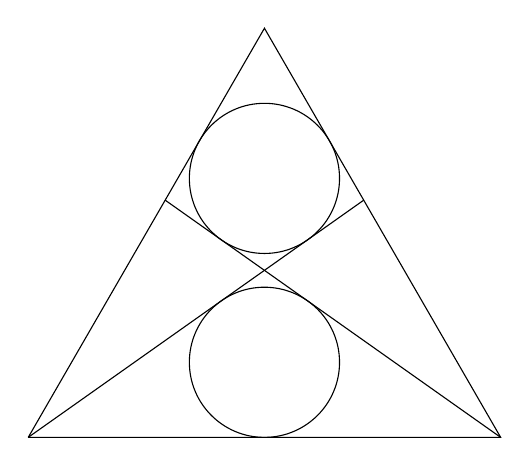
\begin{tikzpicture}[scale=3]

\draw (-1,0) -- (1,0) -- (0, 1.73205) -- (-1,0);
\draw (0,1.09637) circle (0.317837);
\draw (0,0.31783) circle (0.317837);
\draw (-1,0) -- (0.42020,1.0042);
\draw (1,0) -- (-0.42020,1.0042);

\end{tikzpicture}
\end{center}

\section{Putnam and Beyond 1.1.3 (generalizado)}

Sejam $k$ inteiro positivo e $S = \{a_1,a_2,\;\dots,a_n\}$ um conjunto de inteiros positivos primos dois a dois tal que $1<a_i\le k,\; \forall a_i\in S$. Determine o menor $n$ para o qual $S$ contém ao menos um número primo.

\section{Revista do Professor de Matemática 103 problema 453/Dissertação lokona (generalizado)}

Seja $p(x) = x^n + a_{n-1} x^{n-1}+\;\dots+a_1x+a_0$ um polinômio de n raízes reais em que $a_{n-1} = -nk$, para $k$ algum real positivo. Sabendo que $p(k+1) > 1$, prove que $p(x)$ tem ao menos uma raiz maior que $k+1$. 

\section{Revista do Professor de Matemática 103 problema 452 (generalizado)}

Ache os inteiros $n$ tal que $\frac n2 +1$ são quadrados perfeitos.